\documentclass[12pt,a4paper]{ctexart}

\usepackage[UTF8]{ctex}
\usepackage{geometry}
\usepackage{graphicx}
\usepackage{xcolor}
\usepackage{tikz}
\usepackage{fontspec}
\usepackage{setspace}
\usepackage{enumitem}
\usepackage{booktabs}
\usepackage{array}
\usepackage{longtable}
\usepackage{hyperref}
\usepackage{fancyhdr}
\usepackage{titlesec}
\usepackage{multicol}
\usepackage{xurl}
\usepackage{tocloft}

\renewcommand{\cfttoctitlefont}{\hfill\bfseries\Large}
\renewcommand{\cftaftertoctitle}{\hfill}
\geometry{left=2.5cm,right=2.5cm,top=2.5cm,bottom=2.5cm}

\definecolor{black}{RGB}{0,0,0}
\definecolor{mainblue}{RGB}{0,82,147}
\definecolor{accentgold}{RGB}{180,140,60}
\definecolor{lightgray}{RGB}{245,245,245}
\definecolor{darkgray}{RGB}{80,80,80}
\definecolor{mainred}{RGB}{230,1,45}

\hypersetup{
    colorlinks=true,
    linkcolor=black,
    urlcolor=mainblue,
    citecolor=mainblue,
    pdfborder={0 0 0}
}

\pagestyle{fancy}
\fancyhf{}
\fancyhead[L]{\small\color{darkgray}\textbf{量子行业每周新闻洞察}}
\fancyhead[R]{\small\color{darkgray}\textbf{总第194期}}
\fancyfoot[C]{\thepage}
\renewcommand{\headrulewidth}{0.4pt}
\renewcommand{\footrulewidth}{0pt}

\titleformat{\section}
    {\Large\bfseries\color{mainred}}
    {\thesection、}{0em}{}
\titleformat{\subsection}
    {\large\bfseries\color{mainred}}
    {\thesubsection、}{0em}{}

\newcolumntype{L}[1]{>{\raggedright\arraybackslash}p{#1}}
\newcolumntype{C}[1]{>{\centering\arraybackslash}p{#1}}

\begin{document}

% ==================== 封面 ====================
\begin{titlepage}
\begin{tikzpicture}[remember picture,overlay]
    \fill[mainred] ([yshift=-0.5cm]current page.north west) rectangle ([yshift=-1.2cm]current page.north east);
    \fill[mainred] ([yshift=1.2cm]current page.south west) rectangle ([yshift=0.5cm]current page.south east);
\end{tikzpicture}

\vspace*{4cm}

\begin{center}
    {\fontsize{44}{52}\selectfont\bfseries\color{black} \textbf{量子行业每周新闻洞察}}

    \vspace{0.8cm}

    {\fontsize{16}{22}\selectfont\color{darkgray} 2026.08.23 — 2026.08.28 }
    {\fontsize{16}{22}\selectfont\color{darkgray} \textbf{WEEKLY NEWS}}

    \vspace{1.5cm}

    {\fontsize{20}{26}\selectfont\color{mainred}\textbf{（总第\textbf{ 194 }期）}}

    \vspace{4cm}

    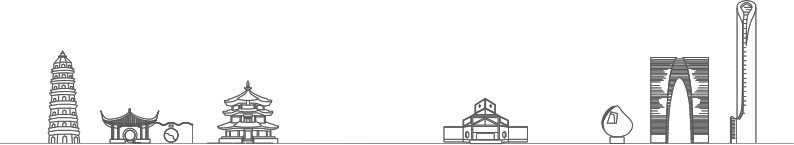
\includegraphics[width=\textwidth]{Cover_Suzhou.png}

    \vfill

    {\fontsize{12}{16}\selectfont\color{darkgray} 量子科技长三角产业创新中心\\编制：科技委办公室、产业发展部（理事会办公室）}
\end{center}
\end{titlepage}

% ==================== 目录 ====================
\pagenumbering{roman}
\newpage
\tableofcontents

\newpage

% ==================== 摘要 ====================
\pagenumbering{arabic}
\setcounter{page}{1}
\begin{center}
{\Large\bfseries\color{mainred} 摘\hspace{2em}要}
\end{center}
\addcontentsline{toc}{section}{摘要}


\textbf{ 宏观态势：}

全球量子技术布局呈现显著的国家战略化特征，欧美日等经济体纷纷通过长周期、大额度的公共资金投入夯实基础研究底座。美国NSF连续多项资助聚焦实用量子纠错与超导制造瓶颈，显示出从实验室原理验证向工程化、可扩展制造转型的明确意图。瑞典发布首份国家级战略及日本部署全栈中性原子计算机，则标志着技术主权竞争正从单一环节突破走向全链条体系建设，量子政策与产业规划的耦合度显著增强。


\textbf{ 科技前沿：}

纠错码与量子比特相干性保真成为突破集中区，Photonic、哈佛等团队侧重以更少的物理资源实现更高容错能力，体现了行业对规模化、低开销纠错路径的迫切追求。同时，真空涨落调控、新型单光子探测器及磁性悬浮架构等方向涌现，表明学界正从材料、器件和物理机制层面多路并进，试图绕开传统超导方案的固有障碍。值得一提的是，剑桥关于“魔法态”门槛的新论证，开始为量子优势的实际边界提供更审慎的理论校准。


\textbf{ 产品动态：}

产品端加速从通用硬件向场景化解决方案渗透，重力导航、量子化学模拟及费米子软件框架等细分工具密集落地，反映行业正为特定行业构筑应用闭环。欧洲公采资金大额招标与韩国的设备研制并举，显示政府作为首次采购方和验证方的角色愈发关键，正推动量子技术跨越早期市场鸿沟。此类项目普遍强调与现有工业流程的兼容性，实用主义导向明显。


\textbf{ 企业资讯：}

产业界呈现“合纵连横”的全球化协作态势，巨头通过并购、联合研发与跨国渠道拓展强化生态位，如IBM收购HRL、Pasqal深耕中东市场均印证地缘战略与商业布局的绑定。企业路线图普遍设定至2030年代初期的集成规模目标，以中长期技术承诺获取资本与政策信任。同时，软件与AI工具（如微软Skala集成）开始成为赋能硬件落地、提升模拟效率的新竞争焦点。


\textbf{ 资本运作：}

本周公开披露的投融资事件相对稀少，仅见个别公共资金对具体企业研发设施的定向支持，整体市场情绪趋于观望。资本活动较前几周明显收缩，可能受假期因素及全球宏观环境不确定性影响。在缺乏大宗交易信号的情况下，行业资金面更依赖政策采购与政府专项拨款维系，市场化风投的配置节奏暂未见显著转向。




\textbf{ 专利动态：}

本周专利动态涵盖低温环境系统、超导量子测控技术、量子软件与算法共3个板块、21条专利。




% ==================== 会议列表 ====================
{
    \newpage
    \section*{ 9月量子科技行业国内、国际会议}
    \addcontentsline{toc}{section}{ 9月量子科技行业国内、国际会议}
    \scriptsize
    \begin{longtable}{C{0.8cm}L{2.5cm}L{3cm}L{7cm}}
        \toprule[1.5pt]
        \textbf{序号} & \textbf{日期} & \textbf{地点} & \textbf{会议名称} \\
        \midrule
        \endfirsthead
        \toprule
        \textbf{序号} & \textbf{日期} & \textbf{地点} & \textbf{会议名称} \\
        \midrule
        \endhead
        \bottomrule
        \endfoot
        
        1 & 9月2日-4日 & 罗马, 意大利 & 量子人工智能在生物信息学与生物统计学中的专题分会：理论、算法与应用 \\
        \midrule[0.05pt]
        
        2 & 9月6日-11日 & 匹兹堡, 美国 & 应用超导会议 2026 (ASC) \\
        \midrule[0.05pt]
        
        3 & 9月7日-10日 & 因斯布鲁克, 奥地利 & Aurora因斯布鲁克量子光子学学校 (AQUARiQ) 2026 \\
        \midrule[0.05pt]
        
        4 & 9月7日-11日 & 波普洛尼亚, 意大利 & 物质波光学前沿暑期学校：称量世界 (FOMO) \\
        \midrule[0.05pt]
        
        5 & 9月9日-10日 & 哥本哈根, 丹麦 & Q2B \\
        \midrule[0.05pt]
        
        6 & 9月9日-11日 & 诺丁汉, 英国 & Quantum Roundabout 量子会议 \\
        \midrule[0.05pt]
        
        7 & 9月13日-18日 & 多伦多, 加拿大 & IEEE量子周 2026 \\
        \midrule[0.05pt]
        
        8 & 9月14日-18日 & 维也纳, 奥地利 & VCQ与quantA暑期学校2026：实现量子优势—从基础到应用 \\
        \midrule[0.05pt]
        
        9 & 9月14日-18日 & 波普洛尼亚, 意大利 & 物质波光学前沿会议 (FOMO) \\
        \midrule[0.05pt]
        
        10 & 9月14日-18日 & 剑桥, 英国 & InQuanto暑期学校 \\
        \midrule[0.05pt]
        
        11 & 9月15日 & 科利奇帕克, 美国 & 量子跃迁职业枢纽 \\
        \midrule[0.05pt]
        
        12 & 9月15日-17日 & 代尔夫特, 荷兰 & 量子信息稀土离子研讨会 (REIQI) \\
        \midrule[0.05pt]
        
        13 & 9月21日 & 多伦多, 加拿大 & 第8届国际量子资源估算研讨会 (QRE) \\
        \midrule[0.05pt]
        
        14 & 9月21日-25日 & 里约热内卢, 巴西 & 2026年巴西量子科学与技术大会 \\
        \midrule[0.05pt]
        
        15 & 9月21日-10月9日 & 维也纳, 奥地利 & 超快电子学与量子热力学交叉暑期学校与研讨会 \\
        \midrule[0.05pt]
        
        16 & 9月22日-23日 & 柏林, 德国 & 量子峰会 \\
        \midrule[0.05pt]
        
        17 & 9月22日-24日 & 科利奇帕克, 美国 & 2026年量子世界大会 \\
        \midrule[0.05pt]
        
        18 & 9月28日-10月17日 & 圣巴巴拉, 美国 & 量子前沿人工智能研讨会 \\
        \midrule[0.05pt]
        
        19 & 9月28日-10月2日 & 帕德博恩, 德国 & 2026量子光子学聚焦 \\
        \midrule[0.05pt]
        
    \end{longtable}
}




% ==================== 宏观态势 ====================
\newpage
\section{宏观态势}
\vspace{-0.5em}
\noindent\rule{\linewidth}{1.5pt}

\subsection{ 美国国家科学基金会资助3750万美元成立实用量子纠错物理与工程研究所 }

2026年08月27日消息，耶鲁大学领导的多学科研究团队获美国国家科学基金会（NSF）3750万美元资助，用于建立NSF量子跃迁挑战·实用量子纠错物理与工程研究所（NSF PRACTIQAL），旨在重新设计实用且可自纠错的量子计算机。该中心为NSF新资助的8项拨款之一，致力于在物理量子比特、控制电子设备、算法运行等层面推进技术突破。研究聚焦两大挑战：一是识别阻碍纠错量子计算机规模化扩展的关键问题，提升量子纠错实用性与效率；二是探索团队首创的“擦除量子比特”，此类特制量子比特可充当标志，精确指示错误发生位置与时间，为高效纠错提供新路径。

\noindent\textbf{报道链接：}\url{https://engineering.yale.edu/news-and-events/news/nsf-grant-yale-leads-effort-develop-practical-industry-scale-quantum-computers}

\subsection{ NSF资助2790万美元成立MARQUIS研究所，攻关超导量子处理器制造瓶颈 }

2026年08月27日消息，美国国家科学基金会宣布资助2790万美元成立新研究所“MARQUIS”（可制造且具有韧性的超导量子信息系统），以加速量子计算的发展。MARQUIS研究所由普林斯顿大学牵头，其他参与机构包括康奈尔大学、麻省理工学院、加州大学圣巴巴拉分校、斯坦福大学、纽约创建大学、密歇根歇根州立大学、爱荷华大学和达特茅斯学院。该所将汇聚多个领域的专家，共同应对量子处理器核心组件制造这一关键瓶颈，并开展硬件制造技术研究，同时开发教育和劳动力培训项目，以加深美国在量子科学与工程领域的领先地位。

\noindent\textbf{报道链接：}\url{https://engineering.dartmouth.edu/news/dartmouth-to-participate-in-nsf-funded-institute-to-meet-quantum-computing-challenges}

\subsection{ NSF续资3750万美元支持HQAN量子飞跃挑战研究所，推进模块化量子计算研究 }

2026年08月27日消息，美国国家科学基金会（NSF）已为伊利诺伊大学厄巴纳-香槟分校牵头的“混合量子架构与网络·量子飞跃挑战研究所”（NSF HQAN）续期第二阶段资助，五年共计将投入3750万美元。该中心专注于研究模块化量子计算方法，即通过网络连接多个小型量子处理单元（QPU）以提升整体计算能力，从而规避直接扩展QPU的技术难题。该中心参与团队包括伊利诺伊大学、芝加哥大学、威斯康星大学麦迪逊分校和西北大学组成，斯坦福大学和MIT林肯实验室提供关键能力支持，第二阶段中心将拥有16个行业合作伙伴，包括 Google、IBM、IonQ和Quantinuum等。

\noindent\textbf{报道链接：}\url{https://grainger.illinois.edu/news/stories/HQAN-renewed-five-years}

\subsection{ 瑞典已发布首个国家量子技术战略，明确到2036年的五大发展目标 }

2026年08月26日消息，瑞典政府已发布该国首个国家量子技术战略，设定到2036年在研究、产业、人才、安全及国际合作方面的发展目标，并呼吁尽早采用包括后量子密码在内的量子安全网络措施，以应对当前加密体系面临的未来威胁。该战略确定了2036年的五个目标，包括强化研究、创新与工业竞争力，保障高水平技能人才供给，加强政府、学术界与产业界的协同，保护并负责任地使用战略性量子技术，以及积极参与国际合作。

\noindent\textbf{报道链接：}\url{https://thequantuminsider.com/2026/08/24/sweden-sets-2036-deadline-for-national-quantum-technology-strategy/}

\subsection{ 美国财政部成立量子安全准备工作组，推动金融业向抗量子密码迁移 }

2026年08月25日消息，美国财政部宣布成立量子安全准备工作组，以落实特朗普总统签署的第14412号行政命令，强化美国敏感数据、关键基础设施及数字经济的加密保护。该小组将助力金融体系在新技术重塑全球格局时维持稳健、安全与竞争力。该任务小组为公私合作机制，旨在以有序且具备运营韧性的方式，加速美国美国金融业向量子安全技术过渡，相关工作基于G7网络专家小组发布的后量子密码迁移路线图。小组下设三条工作线：行业协调与后量子密码迁移、第三方及供应商准备、数字资产与新兴技术风险。此次举措标志着美国金融监管层正将后量子安全议题纳入系统性推进轨道。

\noindent\textbf{报道链接：}\url{https://home.treasury.gov/news/press-releases/sb0615/}

\subsection{ 日本首台全栈中性原子量子计算机启动，Infleqtion提供核心量子处理单元 }

2026年08月25日消息，日本分子科学研究所的一个研究团队在量子计算与量子传感企业Infleqtion的支持下，启动了日本首台可运行的中性原子全栈量子计算机。该系统名为“Shunkai”，初期预计运行约50个量子比特，并计划随开发推进扩展至约500个量子比特。Infleqtion为该平台提供量子处理单元，并以主要研究者身份参与该团队Ohmori教授领导的Moonshot登月项目，以推动该系统从研发阶段迈向实际运行。据悉，Infleqtion也是日本科学技术振兴机构（JST）“量子登月计划”中唯一入选的外国量子合作伙伴。

\noindent\textbf{报道链接：}\url{https://infleqtion.com/infleqtion-collaboration-with-japan-moonshot-program-achieves-major-milestone-shunkai-neutral-atom-quantum-computer-now-operational/}


% ==================== 科技前沿 ====================
\newpage
\section{科技前沿}
\vspace{-0.5em}
\noindent\rule{\linewidth}{1.5pt}

\subsection{ Photonic Inc.发布QLDPC纠错码新成果，SHYPS码能以更少量子比特实现高效计算 }

2026年08月28日消息，加拿大量子计算公司Photonic Inc.宣布，其关于SHYPS量子纠错码的研究论文《QLDPC码的高效计算》已发表在《自然通讯》期刊。该论文报告了Photonic去年以预印本形式发布的里程碑成果：一种名为SHYPS的新型量子低密度奇偶校验（QLDPC）码家族，能够能够以远少于表面码所需的物理量子比特数量，高效执行量子计算与纠错任务。Photonic称，这是业界首次解锁QLDPC码数十年的潜力，为能够运行该类码的量子架构带来了切实益处，树立了新的行业标准。该成果有望缩短量子计算走向商业应用的时间线。

\noindent\textbf{报道链接：}\url{https://photonic.com/news/qldpc-logic-in-naturecomms/}

\subsection{ 哈佛团队成功演示硅空位自旋全机械相干保护，相干时间延长约三倍 }

2026年08月28日消息，哈佛大学约翰·保尔森工程与应用科学学院（SEAS）的研究团队演示了仅使用机械振动来保护脆弱量子信息的新方法，并对金刚石中硅空位自旋进行“全机械相干保护”。与依赖微波脉冲的传统方案不同，他们应用由声子构成的连续机械驱动场，将量子比特转换为“修饰式”（dressed）量子比特，由于它们“包裹”着一个连续的声场，因此对环境中的低频噪声不太敏感。新方法能将硅空位自旋的相干时间延长约三倍，证明连续波机械噪声抑制在真实器件中能够有效延长量子相干时间。相关研究成果已于近日发表在《自然物理学》期刊。

\noindent\textbf{报道链接：}\url{https://seas.harvard.edu/news/qubits-dressed-success}

\subsection{ NIST开发新型超导纳米线单光子探测器：导线宽百倍，暗电流降低十亿倍 }

2026年08月26日消息，美国国家标准与技术研究院（NIST）的物理学家在《Optica》上发表研究，展示了一种超导纳米线单光子探测器（SNSPD）的改进方案：将纳米线宽度扩展至0.1毫米，比传统器件宽100倍以上，并创造了一项新纪录：暗电流降低十亿倍。更宽的导线简化了器件设计与制造流程，使大型探测器阵列更易生产，且能捕获更多光子，尤其适用于光源极微弱、受控程度较低的场景。这一进展有望推动弥散相关光谱法等医疗成像技术，以及用于研究遥远星系微弱低能光信号的天文学观测应用。

\noindent\textbf{报道链接：}\url{https://www.nist.gov/news-events/news/2026/08/nist-researchers-supersize-quantum-technology-help-detect-faint-photons}

\subsection{ 我国科学家首次实验证实真空涨落可增强超导性 }

2026年08月26日消息，中国科学技术大学曾长淦教授、程广珲教授团队联合上海交通大学蒋庆东教授、麻省理工学院Frank Wilczek教授等合作者，首次实验证实真空涨落可增强超导性。团队将超导体NbSe2嵌入太赫兹暗腔，构建了超导体-暗腔耦合器件。团队对比腔内外超导性能发现，NbSe2的超导临界温度显著提升，其中六层器件临界温度最高提升5.4\%，临界电流和临界磁场也明显增强。该研究利用腔工程真空涨落，非侵入式增强超导，无需外部驱动，为量子态调控提供了非接触控制手段。相关研究成果已于日前发表在《自然》期刊。

\noindent\textbf{报道链接：}\url{https://www.eurekalert.org/news-releases/1141207}

\subsection{ 拦截有害光子于超导电路之外，QTREX专利技术有望解决量子比特一大规模化障碍 }

2026年08月25日消息，QTREX Quantum宣布其正在申请一项专利技术，它针对量子计算规模化的一大障碍：杂散辐射会破坏库珀对、产生准粒子、缩短量子比特寿命并推高错误率。该技术利用局部激光处理，首次将3D打印的介电材料直接转化为导电的类石墨烯碳材料，使选定区域的打印绝缘体变为图案化导电结电结构，无需添加导电材料或单独组件组装，即打印绝缘材料本身成为导体。QTREX目前正将该能力集成至量子封装中，作为单片杂散光子吸收器，在有害光子到达超导电路前将其拦截。

\noindent\textbf{报道链接：}\url{https://www.globenewswire.com/news-release/2026/08/19/3347716/0/en/qtrex-s-patent-pending-technology-achieves-first-direct-conversion-of-3d-printed-insulation-into-graphene-like-carbon-to-protect-quantum-processors.html}

\subsection{ 明亮压缩真空光在氩介质中的退相干效应可被抑制 }

2026年08月24日消息，西班牙光子科学研究所（ICFO）与合作伙伴在《自然·通讯》上发表一篇研究，他们考察了明亮压缩真空（BSV）光在氩原子介质中传播时由此产生的退相干效应，并探索了最小化方法。结果表明，BSV驱动的高次谐波产生可能被原子电离和光子损失等副作用掩盖，导致辐射的量子特性退化、最、最大传播长度受限、发射谐波数量减少。不过，该团队证明这些退相干效应并非不可克服：通过显著降低原子电离引起的光子损失，并精确控制BSV强度，可在抑制退相干的同时保留BSV产生高次谐波的能力，从而高效生成具有量子特性的谐波。

\noindent\textbf{报道链接：}\url{https://www.icfo.eu/news/2698/how-to-generate-high-harmonics-with-quantum-light-despite-decoherence/880/}

\subsection{ 哈佛大学与斯图加特大学理论预言菱面体石墨烯中可能出现新型超导态 }

2026年08月24日消息，哈佛大学与斯图加特大学的研究人员在《物理评论快报》上发表一篇论文，理论上证明一种被称为“谷不平衡菱面体四层石墨烯”的特殊材料可承载非常规超导态。该研究发现，尽管材料体系内的不平衡会打破时间反演对称性，谷不平衡仍能支持有限动量、拓扑性质的超导配对。这种材料中的超导性可以可以同时在多个不公度动量处凝聚，从而导致库珀对超晶格的自发形成。这一结果拓展了对拓扑超导与超晶格超导机制的理解，为探索新型量子材料提供了理论依据。

\noindent\textbf{报道链接：}\url{https://phys.org/news/2026-08-unusual-superconductivity-emerge-valley-imbalanced.html}

\subsection{ 研究人员提出新型量子计算架构，通过超导磁悬浮氖粒子规避量子比特表面缺陷 }

2026年08月24日消息，FAMU-FSU工程学院与美国国家高磁场实验室的研究人员设计了一种新型量子计算架构，它利用磁悬浮技术弥补了量子比特制造过程中出现的表面随机缺陷。在电子对-氖量子比特器件中，氖表面的微小凸起容易捕获电子，导致器件行为难以预测。该团队通过利用超导磁体悬浮氖粒子，有效规避了这一稳定性问题。该成果有望为更可重复、可扩展的量子计算技术铺平道路，也为将清洁量子材料直接集成于芯片控制电路的新型混合量子设备开辟了路径。相关研究已于日前发表于美国物理学会期刊《PRX Quantum》。

\noindent\textbf{报道链接：}\url{https://news.fsu.edu/news/science-technology/2026/08/20/famu-fsu-college-of-engineering-researchers-design-magnetically-levitated-quantum-bit/}

\subsection{ 剑桥大学新研究揭示量子优势更高门槛：仅有“魔法态”并不足够 }

2026年08月24日消息，剑桥大学卡文迪什实验室领导的一项新理论研究显示，量子计算机实现强大计算能力的难度要高于此前预期，并更清晰地刻画了真正使其发挥作用的条件。该团队识别出了对量子计算真正有用的精确量子态，同时扩大了经典计算机能够轻松计算的量子计算范围，这意味着量子设备要想展示相对于经典计算机的“量子优势”，需跨越更高门槛。该研究证明“魔法态”是解锁量子计算机全部能力的必要条件，但也并不充分。如果量子态没有“魔法”，就不可能获得量子优势；但仅有“魔法”也不能保证能获得优势。相关成果已于日前发表在《物理评论快报》上。

\noindent\textbf{报道链接：}\url{https://www.phy.cam.ac.uk/news/a-little-bit-more-than-magic-the-secret-to-quantum-computing-may-lie-in-negativity/}


% ==================== 产品动态 ====================
\newpage
\section{产品动态}
\vspace{-0.5em}
\noindent\rule{\linewidth}{1.5pt}

\subsection{ SandboxAQ以量子化学计算驱动的大型定量模型登陆亚马逊AWS云市场 }

2026年08月28日消息，SandboxAQ宣布其大型定量模型（LQM）AQCat正式在亚马逊AWS Marketplace上架，并可通过Amazon SageMaker部署。该模型面向材料创新者、工业企业及研发团队，用户可在自有AWS环境中直接运行，无需配备专业计算科学家或编写自定义代码。A。AQCat基于47000个催化剂系统的1350万次高保真量子化学计算训练而成，能以最高达传统物理方法20000倍的速度预测决定催化剂性能的关键属性，同时接近传统方法的准确性。企业可借此对海量候选材料进行计算筛选和排序，将昂贵的实验室与超算资源集中于最具潜力的方向，从而压缩研发周期并降低投资风险。

\noindent\textbf{报道链接：}\url{https://www.sandboxaq.com/press/sandboxaq-aqcat-aws-marketplace}

\subsection{ Q-CTRL完成全球首次海上实地演示无GPS量子重力导航 }

2026年08月28日消息，量子基础设施软件领导者Q-CTRL宣布，它已在澳大利亚东海岸成功利用软件加固型量子重力仪实现海上船只无GPS自主导航的全球首次实地演示。在一系列试验中，该公司实现了自主重力测绘和无GPS量子重力导航，并达到1海里定位精度。该演示基于Q-CTRL的新一代量子定位导航系统系统Ironstone Opal，它通过感知地球独特的地球物理特征提供类似GPS的定位能力，可适用于空中、陆地、海上等场景，能在GPS不可用或受干扰时作为可靠备用。该系统能全天候运行，不依赖收发外部无线电信号，因此可抵御信号干扰与欺骗攻击。

\noindent\textbf{报道链接：}\url{https://q-ctrl.com/blog/q-ctrl-achieves-worlds-first-gps-free-quantum-gravimetric-navigation-demonstration-in-maritime-field-trial}

\subsection{ 欧洲EuroHPC JU启动6项新量子技术招标 总经费达1.19亿欧元 }

2026年08月26日消息，欧洲高性能计算联合体EuroHPC JU已发起六项新招标，总额达1.19亿欧元，旨在推动欧洲下一代量子系统的研发与部署。招标的量子计算路线涵盖离子阱、超导和中性原子三条技术路线，分别要求开发1000+可寻址物理量子比特的全栈离子阱系统、基于芯片技术且具有1000+可单独寻址物理量子比特的超导量子处理器，以及具有10000个用于模拟的原子和1000个物理比特的可编程中性原子平台。同时，招标还涉及下一代量子密钥分发系统，要求城域密钥率超1Mbps、区域网络覆盖超300公里，并探索QKD与后量子密码融合方案。另外两项分别是泛欧开放式量子测试基础设施和量子实验试点线建设。

\noindent\textbf{报道链接：}\url{https://www.eurohpc-ju.europa.eu/six-new-quantum-calls-launched-eurohpc-joint-undertaking-2026-08-14\_en}

\subsection{ IBM发布Qiskit Fermions，填补费米子模拟量子软件框架空白 }

2026年08月26日消息，IBM发布了一项新的开源研究能力Qiskit Fermions，为量子软件生态提供专注于费米子系统的灵活框架。该工具可直接处理费米子系统，支持表达费米子算符和电路、定义费米子到量子比特的映射，并将费米子工作流编译为量子电路。IBM表示，创建该工具旨在填补量子软件生态系态系统中缺乏专用现代框架的空白，同时希望构建一个能够满足多样研究需求的多功能工具箱。作为面向费米子体系量子模拟的软件组件，Qiskit Fermions有望为研究人员提供全方位的需求和用例服务。

\noindent\textbf{报道链接：}\url{https://www.ibm.com/quantum/blog/qiskit-fermions}

\subsection{ 韩国正开发量子重力仪和量子显微镜 瞄准潜艇导航与超精密成像 }

2026年08月24日消息，韩国科学家正致力于将量子技术应用于量子重力仪和超精密显微镜等领域。韩国标准科学研究院（KRISS）的一个原子量子传感研究组正在研发量子重力仪，目标是在2032年前推出可安装于实际潜艇的原型机，以用于修正潜艇水下位置。目前该团队在实验室层面已实现世界级灵敏度。与此同时，韩国电子通信研究院（ETRI）正推进量子显微镜商业化研究，其分辨率高于传统光学显微镜，这种显微镜即使在光线较弱的情况下，也能实现比传统光学显微镜更高的分辨率和灵敏度。

\noindent\textbf{报道链接：}\url{https://www.dongascience.com/en/news/79491}



% ==================== 专利动态 ====================
\newpage
\section{专利动态}
\vspace{-0.5em}
\noindent\rule{\linewidth}{1.5pt}

\subsection{ 低温环境系统 }

\subsubsection{ 利用超导刚挠性电路在量子比特表面和量子比特表面控制系统之间维持高热梯度的系统和方法。 }

申请人：微软技术许可有限责任公司

发明人：ターナー,マシュー デイビッド | ランタ,クレイグ スティーブン | クレイマー,ケビン ジェームス

公开日/授权日：2026-08-26

摘要：

本文描述了一种用于在量子比特表面和量子比特表面控制系统之间维持高热梯度的系统和方法。该系统包括与超导刚挠性电路的第一刚性电路部分关联的量子比特表面,以及与该超导刚挠性电路的第二刚性电路部分关联的控制系统。该超导刚挠性电路包括用于连接第一刚性电路部分和第二刚性电路部分的柔性电路部分。该系统还包括第一冷却系统,其能够将量子比特表面和超导刚挠性电路的第一刚性电路部分的工作温度维持在100毫开尔文以下。该系统还包括控制系统和第二冷却系统,其能够将超导刚挠性电路的第二刚性电路部分的工作温度维持在10开尔文以下。

\noindent\textbf{专利链接：}\url{https://analytics.zhihuiya.com/patent-view/abst?patentId=f09696bb-8816-4864-a2c1-3f0831f74505&shareId=F0B99893-G204-5B3D-209G-6B3G48021D31&from=EXPORT&signature=0exuMOqA5gaxVMS487H2VnybrcRxjsaiNFRkCZV520Y%3D&expire=94608000&date=20260828T063441Z&version=1.0}

\subsubsection{ 一种具有宽温域压卡效应的复合量子点温度记忆材料及其制备方法和应用 }

申请人：二四九五企业管理(珠海)有限公司

发明人：梁海 | 胡艳梅

公开日/授权日：2026-08-25

摘要：

本发明公开了一种具有宽温域压卡效应的复合量子点温度记忆材料及其制备方法和应用，属于温控材料技术领域。该复合量子点温度记忆材料为碳量子点/压卡塑晶材料复合物，其具有能在温度变化时发生可逆性畸变的晶格结构，所述可逆性畸变为：当温度升高时，晶格扩张，吸收外界热量；当温度降低时，晶格收缩，释放储存的热量。该材料通过吸放热循环，并依托压卡效应实现‑80℃\textasciitilde{}300℃全温区精准温度记忆，温区覆盖范围广，在极端温度下无脆裂、无分解、无性能衰减，压卡效应稳定，温度记忆误差不超过±1℃，能适配于多种不同成型方式，能很好地满足建筑陶瓷、制冷板材、建筑墙面、工业设备、汽车表面、温控零部件等不同应用场景的使用需求。

\noindent\textbf{专利链接：}\url{https://analytics.zhihuiya.com/patent-view/abst?patentId=dc3036ca-3eac-4d77-8d83-851d81bd4963&shareId=F0B99893-G204-5B3D-209G-6B3G48021D31&from=EXPORT&signature=NtmkojEFFHucszTPYOjn5Xk1rrF0gAgJuKJJt2AGmwk%3D&expire=94608000&date=20260828T063441Z&version=1.0}

\subsubsection{ 全封闭式微流压力控制系统及方法 }

申请人：中国科学院理化技术研究所 | 北京石油化工学院

发明人：高波 | 韩东旭 | 宇波 | 王齐 | 孙东亮 | 张海洋 | 孔祥杰

公开日/授权日：2026-08-25

摘要：

本发明提供一种全封闭式微流压力控制系统及方法，涉及深低温计量与精密压力控制技术领域，该系统包括第一低温恒温器和第二低温恒温器；连通管路，连接两个恒温器的气相空间，构成全封闭气体回路；气体流量控制阀门，设置于连通管路上；主动控温单元，与第二低温恒温器热耦合；中央控制系统，用于根据第一低温恒温器的实际压力与目标压力的偏差，控制主动控温单元调节第二低温恒温器的温度以产生压差，并根据偏差控制气体流量控制阀门的开度，使工作气体在全封闭气体回路中转移，以调节第一低温恒温器的内部压力。本发明实现了工作气体的零损耗循环利用，适用于极低温物理实验、量子计算及低温恒温器等应用场景中的高精度压力控制。

\noindent\textbf{专利链接：}\url{https://analytics.zhihuiya.com/patent-view/abst?patentId=07e972eb-1196-40f9-b6f1-bfcd0f5905b6&shareId=F0B99893-G204-5B3D-209G-6B3G48021D31&from=EXPORT&signature=ZfXNz42H5rbaimAtbqpNRKox0%2B2%2FA7MrsdsKpS6%2BbQw%3D&expire=94608000&date=20260828T063441Z&version=1.0}

\subsubsection{ 分布式热管理架构 }

申请人：高通股份有限公司

发明人：ルイ、ルイ | アルトン、ロナルド | ウィリアム、スマリン | メへトレ、ビナヤック·ナナ

公开日/授权日：2026-08-25

摘要：

该热管理配置包括串行数据总线、中央处理器 (CPU)、图形处理器 (GPU)、神经信号处理器 (NSP) 和始终开启子系统 (AOSS),所述串行数据总线、CPU、GPU、NSP 和 AOSS 均在片上系统 (SoC) 上实现,所述 CPU 包括第一组热传感器和第一组控制器,所述第一组热传感器分别与所述第一组控制器耦合,所述 NSP 包括第二组热传感器和第二组控制器,所述第二组热传感器分别与所述第二组控制器耦合,所述 AOSS 包括第三组热传感器和第三组控制器,所述第三组热传感器分别与所述第三组控制器耦合。

\noindent\textbf{专利链接：}\url{https://analytics.zhihuiya.com/patent-view/abst?patentId=9e525ecd-ec72-457f-87bd-e62d957e01dd&shareId=F0B99893-G204-5B3D-209G-6B3G48021D31&from=EXPORT&signature=aSfBPlQNyidymusHNeE6bS1zW4%2FxWbFhLk4UMzjPgbg%3D&expire=94608000&date=20260828T063441Z&version=1.0}

\subsubsection{ 处理器组装、量子计算设备和方法 }

申请人：IQM芬兰公司

发明人：사이라 올리-펜티 | 오르지아치 장-룩 | 라틴마키 파시

公开日/授权日：2026-08-25

摘要：

一种用于量子计算机的处理器组件包括载体、安装在载体上的至少一个量子处理器芯片以及与载体热接触的第一热锚点。该组件还包括第一电连接器和电信号连接,该电信号连接的第一端与载体电连接,第二端与第一电连接器电连接。该处理器组件还包括第二热锚点。第二热锚点与第一热锚点热隔离,并且第二热锚点与第一电连接器热接触。

\noindent\textbf{专利链接：}\url{https://analytics.zhihuiya.com/patent-view/abst?patentId=afa45580-d889-434e-8bc4-b28f285c8eba&shareId=F0B99893-G204-5B3D-209G-6B3G48021D31&from=EXPORT&signature=jVudAUQGTXmDcdJjsHp%2FNIGKdD7l8OkY1cbULi6SSAY%3D&expire=94608000&date=20260828T063441Z&version=1.0}


\subsection{ 超导量子测控技术 }

\subsubsection{ 利用超导刚挠性电路在量子比特表面和量子比特表面控制系统之间维持高热梯度的系统和方法。 }

申请人：微软技术许可有限责任公司

发明人：ターナー,マシュー デイビッド | ランタ,クレイグ スティーブン | クレイマー,ケビン ジェームス

公开日/授权日：2026-08-26

摘要：

本文描述了一种用于在量子比特表面和量子比特表面控制系统之间维持高热梯度的系统和方法。该系统包括与超导刚挠性电路的第一刚性电路部分关联的量子比特表面,以及与该超导刚挠性电路的第二刚性电路部分关联的控制系统。该超导刚挠性电路包括用于连接第一刚性电路部分和第二刚性电路部分的柔性电路部分。该系统还包括第一冷却系统,其能够将量子比特表面和超导刚挠性电路的第一刚性电路部分的工作温度维持在100毫开尔文以下。该系统还包括控制系统和第二冷却系统,其能够将超导刚挠性电路的第二刚性电路部分的工作温度维持在10开尔文以下。

\noindent\textbf{专利链接：}\url{https://analytics.zhihuiya.com/patent-view/abst?patentId=f09696bb-8816-4864-a2c1-3f0831f74505&shareId=07BG8958-DG59-7CG7-CG97-9010C6F472GB&from=EXPORT&signature=anTs3q%2B3y0ErX5vYQ2ejc94CCYrVY03gELPlewhSe78%3D&expire=94608000&date=20260828T063251Z&version=1.0}

\subsubsection{ 一种多比特可扩展量子测控系统 }

申请人：成都中微达信科技有限公司

发明人：邹小波 | 林海川 | 曾耿华 | 王渊

公开日/授权日：2026-08-25

摘要：

本发明公开了一种多比特可扩展量子测控系统，在该系统中，量子测控单元、时钟分发单元和触发分发单元均可根据需要测量与控制的量子比特数量进行相应扩展，并通过数据传输网络与上位机进行通信交互，实现量子测控的相关工作；由于量子测控单元的时钟信号和触发信号由时钟分发单元和触发分发单元提供，且时钟分发单元和触发分发由于均是一路输入多路输出，能够通过级联实现大规模的扩展。因此，本发明通过单独地设置时钟分发单元和触发分发单元来为众多的量子测控单元提供时钟信号和触发信号，能够使同步性更加稳定，可提高量子测控的保真度，适用于大规模量子比特扩展的量子测控场景。

\noindent\textbf{专利链接：}\url{https://analytics.zhihuiya.com/patent-view/abst?patentId=70d3a2af-0890-42d6-871b-abd15755d8e3&shareId=07BG8958-DG59-7CG7-CG97-9010C6F472GB&from=EXPORT&signature=QDn%2BZBN3fM4gIUDAHzIVU68Ln40%2Fh6n0Tp3NcLUvAR0%3D&expire=94608000&date=20260828T063251Z&version=1.0}

\subsubsection{ 内外部时钟信号自动切换电路、超导量子比特测控系统及其发射单元和量子计算装置 }

申请人：深圳量旋科技有限公司

发明人：俞圣 | 邹宏洋

公开日/授权日：2026-08-25

摘要：

本发明公开了一种内外部时钟信号自动切换电路、超导量子比特测控系统及其发射单元和量子计算装置。所述内外部时钟信号自动切换电路包括：时钟信号检测电路和通道开关芯片；时钟信号检测电路检测是否有接入外部时钟信号，若检测到接入，将外部时钟信号转换成第一电压信号，将第一电压信号转换成光能并将光电耦合得到的第一控制信号输出给通道开关芯片；反之，将第二控制信号输出给通道开关芯片；通道开关芯片根据输入的第一控制信号或第二控制信号，在两个时钟信号通道之间进行切换，输出对应的内部时钟信号或者外部时钟信号。本发明将输入的内外部时钟信号有可能的干扰噪声隔断在前端，避免了对系统时钟信号的干扰，保证了系统时钟信号的质量。

\noindent\textbf{专利链接：}\url{https://analytics.zhihuiya.com/patent-view/abst?patentId=dd269058-c73f-4de7-9b32-997c2dad1a02&shareId=07BG8958-DG59-7CG7-CG97-9010C6F472GB&from=EXPORT&signature=YUDyY0AplfcPWKZVsKOItJlzH5LAKR8sHHUo603aciE%3D&expire=94608000&date=20260828T063251Z&version=1.0}

\subsubsection{ 一种扩展量子测控AWG数据波形长度的方法 }

申请人：成都中微达信科技有限公司

发明人：于海 | 张子墨 | 黄守伟 | 吴方

公开日/授权日：2026-08-25

摘要：

本发明公开了一种扩展量子测控AWG数据波形长度的方法，涉及超导量子计算测控技术领域，步骤1，确定目标频率、采样率、带通滤波器参数及原始存储深度；步骤2，按目标频率与采样率比值选内插模式，基础采样率为目标的1/2；步骤3，用DDS生成脉冲样点，14bit有效数据16bit存储，CRC校验并加窗抑制旁瓣；步骤4，低延迟内插扩展样点至2倍，延迟≤5ns；步骤5，DAC开MIX模式，触发同步，串联滤波器滤镜像；步骤6，验证时长、功率与失真度，不达标则调整。本发明无额外硬件成本，低延迟适配量子反馈，AWG波形时长翻倍，信号质量好，兼容多采样率与频率范围，FPGA资源开销小，适配长寿命量子芯片。

\noindent\textbf{专利链接：}\url{https://analytics.zhihuiya.com/patent-view/abst?patentId=24645002-e82f-4cb4-afef-736d32a16b41&shareId=07BG8958-DG59-7CG7-CG97-9010C6F472GB&from=EXPORT&signature=YO46TUfj%2BV9op851QovUYQSMum7J0Oh658Cp1AfqjVc%3D&expire=94608000&date=20260828T063251Z&version=1.0}

\subsubsection{ 一种量子脉冲控制方法、装置及电子设备和存储介质 }

申请人：深圳量旋科技有限公司

发明人：叶惺 | 孟铁军

公开日/授权日：2026-08-25

摘要：

本申请公开了一种量子脉冲控制方法、装置及设备和存储介质，应用于控制器，该方法包括：获取量子测控任务中每个脉冲通道的脉冲时间长度，并获取可编程逻辑器件中每个缓存通道的最大缓存脉冲时间长度；根据各脉冲通道的脉冲时间长度与各缓存通道的最大缓存脉冲时间长度生成资源分配表，资源分配表用于描述每个脉冲通道的脉冲波形数据与至少一个缓存通道之间的缓存映射关系；将资源分配表与各脉冲通道的脉冲波形数据发送至可编程逻辑器件，以使可编程逻辑器件根据缓存映射关系将各脉冲通道的脉冲波形数据存储至对应的缓存通道。本申请在不改变硬件资源的前提下，提高了可编程逻辑器件内部的缓存资源利用率，满足更长退相干时间的量子比特操控需求。

\noindent\textbf{专利链接：}\url{https://analytics.zhihuiya.com/patent-view/abst?patentId=c5ad60c5-c773-4997-9155-8ab5d08724c6&shareId=07BG8958-DG59-7CG7-CG97-9010C6F472GB&from=EXPORT&signature=D%2FPO%2B4bnkjva0W9VZ5dMQYNt%2FMa1Q2uRTYnD7xoR7oc%3D&expire=94608000&date=20260828T063251Z&version=1.0}

\subsubsection{ 能级差估计程序、能级差估计方法和量子计算系统 }

申请人：富士通株式会社 | 株式会社QUNASYS

发明人：松本 徳文 | 中川 裕也 | 日▲高▼ 裕一朗

公开日/授权日：2026-08-25

摘要：

降低量子电路的深度。 

 【解决方案】处理单元 12 使量子计算机 20 执行量子电路 30。量子电路 30 包括第一极性的第一控制门 32 和第二极性的第二控制门 33,每个控制门均由一个辅助量子比特控制。第一控制门 32 将对应于哈密顿量 H(λ) 的第一时间演化算符应用于对应于量子态 |ψ> 的一组量子比特。第二控制门 33 将对应于 H(λ+δλ) 的第二时间演化算符应用于同一组量子比特。处理单元 12 从量子计算机 20 获取一个概率振幅,该概率振幅对应于将两种时间演化算符应用于量子态 |ψ> 的结果匹配 |ψ> 的事件。处理单元 12 通过使用概率幅值执行离散傅里叶变换来获得 H(λ) 和 H(λ+δλ) 能级差的累积分布函数 40,并根据累积分布函数 40 估计差值。

\noindent\textbf{专利链接：}\url{https://analytics.zhihuiya.com/patent-view/abst?patentId=61ae8ba9-7294-4370-a665-68e2d8b45361&shareId=07BG8958-DG59-7CG7-CG97-9010C6F472GB&from=EXPORT&signature=gmfKAcYqhjVbj2Qu3jfqWEHTdmajQqeaALg3yRrKqec%3D&expire=94608000&date=20260828T063251Z&version=1.0}

\subsubsection{ 应用于量子态的量子门的控制哈密顿量 }

申请人：아이디어드 에스엘

发明人：알바레다 피케르, 기예르모 | 브라콘스 아스파치스, 마리오나 | 센티스 에레라, 가엘 | 라모스 베니테스, 헤수스 라몬 | 우르젤 우예, 누리아 | 알시나 코위, 마르크 | 루비오 준코사, 마르셀

公开日/授权日：2026-08-25

摘要：

本发明提供了一种计算机实现的方法,用于确定应用于至少一个量子态的量子门 G 的控制哈密顿量。本发明还提供了根据所述控制哈密顿量驱动的量子系统。

\noindent\textbf{专利链接：}\url{https://analytics.zhihuiya.com/patent-view/abst?patentId=5396a2c5-5e4b-4c72-90a2-49030502cf58&shareId=07BG8958-DG59-7CG7-CG97-9010C6F472GB&from=EXPORT&signature=cv7eRuYKKE5BhXDnEUYDhGNQV8%2BY4JxOsDCTlTSlBgQ%3D&expire=94608000&date=20260828T063251Z&version=1.0}

\subsubsection{ 具有交替布局和屏蔽门的量子点器件 }

申请人：英特尔公司

发明人：GEORGE, HUBERT C. | PILLARISETTY, RAVI | CLARKE, JAMES S.

公开日/授权日：2026-08-25

摘要：

本发明公开了一种量子点器件,其具有与单行有源量子比特关联的交替排列的读取器件,并且可选地,还具有一个或多个屏蔽门。一种具有交替排列布局的量子点器件示例包括:位于有源量子比特行一侧、靠近有源量子比特行第一部分的第一读取器件,用于检测/读取有源量子比特行第一子集的量子态;以及位于有源量子比特行另一侧、靠近有源量子比特行第二部分的第二读取器件,用于检测/读取有源量子比特行第二子集的量子态。屏蔽门可以设置在与读取器件和有源量子比特行耦合的各个门之间,以控制有源量子比特行的量子比特与读取器件之间以及不同读取器件之间的静电相互作用。

\noindent\textbf{专利链接：}\url{https://analytics.zhihuiya.com/patent-view/abst?patentId=07e58803-234c-4724-a0bb-dec439b04b41&shareId=07BG8958-DG59-7CG7-CG97-9010C6F472GB&from=EXPORT&signature=N9RJceluh1tsmZDIufqUg60CPoz0TTVJ%2BdjaVNIqhYo%3D&expire=94608000&date=20260828T063251Z&version=1.0}


\subsection{ 量子软件与算法 }

\subsubsection{ 用于贝叶斯推断的混合量子-经典计算机,采用工程似然函数实现稳健的振幅估计 }

申请人：札帕塔运算股份有限公司

发明人：WANG, GUOMING | KOH, ENSHAN DAX | JOHNSON, PETER D. | CAO, YUDONG | DALLAIRE-DEMERS, PIERRE-LUC

公开日/授权日：2026-08-26

摘要：

混合量子-经典(HQC)计算机利用现有的量子相干性,最大限度地提升噪声量子器件的采样能力,与VQE相比,显著减少了测量次数和运行时间。HQC计算机的灵感来源于量子计量学、相位估计以及最新的“α-VQE”方案,最终形成了一种对误差具有鲁棒性且无需辅助量子比特的通用公式。HQC计算机采用“工程似然函数”(ELF)进行贝叶斯推断。随着物理硬件从噪声中等规模量子计算机过渡到量子纠错量子计算机,ELF形式进一步增强了采样方面的量子优势。这项技术加速了许多量子算法的核心组件,其应用领域涵盖化学、材料、金融等诸多方面。

\noindent\textbf{专利链接：}\url{https://analytics.zhihuiya.com/patent-view/abst?patentId=724774ae-d754-41fc-bb0c-b0b3dcad8082&shareId=F2GF84E7-1GC8-8BEF-B765-D6399653BCG0&from=EXPORT&signature=7biYqFZmj%2FcSzcaKURqMTyBdBpSWhhGcEJKhIxW9wZk%3D&expire=94608000&date=20260828T063351Z&version=1.0}

\subsubsection{ 用于大容量车辆路径问题(CVRP)的混合经典-量子系统 }

申请人：尤尼西斯公司

发明人：SINNO, SALVATORE | MOTT, ALAN | SAHOO, ARATI | FERNANDO D, ANTONIO DAUPHIN | THURAVAKKATH, SHRUTHI

公开日/授权日：2026-08-26

摘要：

用于改进车辆路径规划的混合经典-量子系统采用了遗传算法、模拟退火和量子退火的组合。该混合方法可以进一步探索容量受限车辆路径问题 (CVRP) 的解空间,从而确定改进的路径规划结果。首先对节点(即位置)进行聚类,然后通过遗传算法处理节点簇以确定潜在解。使用模拟退火对潜在解进行演化,生成演化解,每个解都包含演化节点簇。选择一个演化解。所选演化解的每个演化节点簇分别由量子退火器进行退火,以确定穿过演化节点簇的最佳路径。

\noindent\textbf{专利链接：}\url{https://analytics.zhihuiya.com/patent-view/abst?patentId=22160571-9273-4db4-83cc-313b5fd9ba78&shareId=F2GF84E7-1GC8-8BEF-B765-D6399653BCG0&from=EXPORT&signature=ctWXqXKP88wMLmZeEjtE825ODYCvi3TfOUaPH1cCET0%3D&expire=94608000&date=20260828T063351Z&version=1.0}

\subsubsection{ 用于求解数字-模拟量子计算中的优化问题的进化方法 }

申请人：KIPU QUANTUM GMBH

发明人：SIMEN ALBINO, ANTON | HEGADE, NARENDRA NARAYANA | DE OLIVEIRA, MURILO | KUMAR, SHUBHAM | FÜCHSEL, GERNOT | SOLANO, ENRIQUE

公开日/授权日：2026-08-26

摘要：

本发明涉及一种计算机实施的方法,用于使用多量子位系统中的数字模拟量子计算(DAQC)操作来解决给定量子硬件的优化问题。

\noindent\textbf{专利链接：}\url{https://analytics.zhihuiya.com/patent-view/abst?patentId=336cd780-97ae-4e13-a91b-0b80f0216285&shareId=F2GF84E7-1GC8-8BEF-B765-D6399653BCG0&from=EXPORT&signature=ZSF6zg6Ya1Kiaee9KP0Y0Z0oqCfmF0uqtxl73AUoJtk%3D&expire=94608000&date=20260828T063351Z&version=1.0}

\subsubsection{ 一种用于逼近一组偏微分方程中至少两个未知变量的计算机实现方法、混合计算系统、计算机程序产品和计算机可读介质 }

申请人：特拉量子股份公司

发明人：SAGINGALIEVA, ASEL | MELNIKOV, ALEXEY

公开日/授权日：2026-08-26

摘要：

本发明涉及一种计算机实现的、利用量子物理信息神经网络(100)逼近一组偏微分方程的至少两个未知变量(10)的方法,该方法包括以下步骤:提供一个数值网格(20),该网格具有待逼近未知变量(10)的网格坐标(30);提供一个量子物理信息神经网络(100),该量子物理信息神经网络(100)包含一个针对每个未知变量(10)的混合网络(110),其中,各混合网络(110)彼此不互连,每个混合网络(110)具有一个量子网络(120)和一个经典网络(140),其中,该量子网络(120)和该经典网络(140)彼此不互连;将网格坐标 (30) 输入到量子物理信息神经网络 (100) 中,使得网格坐标 (30) 成为每个混合网络 (110) 的输入;并计算每个混合网络 (110) 在每个网格坐标 (30) 处的输出 (Hout),每个输出 (Hout) 对应于网格坐标 (30) 处待近似的不同未知变量 (10),其中每个混合网络 (110) 的输出 (Hout) 是通过组合该混合网络 (110) 的相应量子网络的输出 (Qout) 和相应经典网络的输出 (Cout) 而获得的。本发明还涉及一种混合计算系统、一种计算机程序产品和一种计算机可读介质。

\noindent\textbf{专利链接：}\url{https://analytics.zhihuiya.com/patent-view/abst?patentId=359ae51c-53a9-4702-bd69-4b2481c42204&shareId=F2GF84E7-1GC8-8BEF-B765-D6399653BCG0&from=EXPORT&signature=FSnWioP6vw5mMY0BjKrxgC790HVsc%2B5%2ByLHmDEquWxE%3D&expire=94608000&date=20260828T063351Z&version=1.0}

\subsubsection{ 用于量子物体限制器件的混合架构 }

申请人：昆媞努姆有限責任公司

发明人：デイヴィッド·ヘイズ | アレクサンダー·チェルノグゾフ | カーティス·ヴォーリン | ラッセル·ピー·スタッツ | ジョン·パグヌッチ·ゲーブラー | クリストファー·イー·ランガー

公开日/授权日：2026-08-26

摘要：

本发明提供一种约束装置,其包括一个或多个分选区和一个计算区。每个分选区包括多个分选区射频(RF)导轨,这些导轨限定多个分选约束区域,当施加分选区射频(RD)电压时,这些约束区域用于约束量子物体。每个分选区射频导轨在垂直于其纵轴的方向上具有分选厚度。计算区包括多个计算区射频导轨,这些导轨限定多个计算约束区域,当施加计算区射频电压时,这些约束区域用于约束量子物体。每个计算区射频导轨在垂直于其纵轴的方向上具有计算厚度。计算厚度大于分选厚度。

\noindent\textbf{专利链接：}\url{https://analytics.zhihuiya.com/patent-view/abst?patentId=4c357924-dacb-4311-abfc-ff8bf4037b03&shareId=F2GF84E7-1GC8-8BEF-B765-D6399653BCG0&from=EXPORT&signature=zE2W6U0qWjl%2FNp3omIcahGgci3UJF1w9KbJ4Nfo%2Fw8Y%3D&expire=94608000&date=20260828T063351Z&version=1.0}

\subsubsection{ 一种在量子计算机中引入魔态的方法及量子计算机 }

申请人：汉阳大学校ERICA产学协力团

发明人：권영헌 | 김영훈 | 김한솔 | 최원재

公开日/授权日：2026-08-26

摘要：

本实施例提供了一种在量子计算机中引入魔态的方法,所述量子计算机中,纠错码包括以下步骤:使用重型六边形结构纠错码配置逻辑量子比特,该纠错码通过在四个数据量子比特和一个伴随式量子比特之间引入两个或多个标志量子比特,从两侧连接两个数据量子比特和一个伴随式量子比特;以及对所述逻辑量子比特执行逻辑运算,其中,所述纠错码执行魔态注入过程,将物理量子比特中实现的魔态映射到逻辑态。

\noindent\textbf{专利链接：}\url{https://analytics.zhihuiya.com/patent-view/abst?patentId=b6aa7f64-10cc-48f5-a42f-0cd62d4dc3f7&shareId=F2GF84E7-1GC8-8BEF-B765-D6399653BCG0&from=EXPORT&signature=zpNbAJIWG9gU9zRGNcKmQlHmr7nqmVH9UW%2BJ0XnYx6E%3D&expire=94608000&date=20260828T063351Z&version=1.0}

\subsubsection{ 一种多比特可扩展量子测控系统 }

申请人：成都中微达信科技有限公司

发明人：邹小波 | 林海川 | 曾耿华 | 王渊

公开日/授权日：2026-08-25

摘要：

本发明公开了一种多比特可扩展量子测控系统，在该系统中，量子测控单元、时钟分发单元和触发分发单元均可根据需要测量与控制的量子比特数量进行相应扩展，并通过数据传输网络与上位机进行通信交互，实现量子测控的相关工作；由于量子测控单元的时钟信号和触发信号由时钟分发单元和触发分发单元提供，且时钟分发单元和触发分发由于均是一路输入多路输出，能够通过级联实现大规模的扩展。因此，本发明通过单独地设置时钟分发单元和触发分发单元来为众多的量子测控单元提供时钟信号和触发信号，能够使同步性更加稳定，可提高量子测控的保真度，适用于大规模量子比特扩展的量子测控场景。

\noindent\textbf{专利链接：}\url{https://analytics.zhihuiya.com/patent-view/abst?patentId=70d3a2af-0890-42d6-871b-abd15755d8e3&shareId=F2GF84E7-1GC8-8BEF-B765-D6399653BCG0&from=EXPORT&signature=nM5DGXzZRDvLt6JnuiRFRvUPULFErzi3Oeg3JQBN6q0%3D&expire=94608000&date=20260828T063351Z&version=1.0}

\subsubsection{ 经典增强变分量子本征求解器 }

申请人：札帕塔运算股份有限公司

发明人：RADIN, MAXWELL D. | JOHNSON, PETER D.

公开日/授权日：2026-08-25

摘要：

本发明提供了一种利用经典增强型变分量子本征求解器(VQE)估计费米子哈密顿量基态和激发态能量的方法和系统。所公开的技术克服了先前VQE方法的缺点,即需要大量的电路重复和过长的运行时间才能达到精度,尤其是在使用噪声中等规模量子(NISQ)器件实现时。本发明公开的经典增强型VQE利用经典方法估计期望值。量子计算机无需制备试探态,而是利用试探态与目标态的经典可处理近似之间的差异。基态能量估计速度显著提高。此外,仅使用基态与用于增强的计算基态之间的重叠,即可估计传统VQE单基态增强的测量减少量。

\noindent\textbf{专利链接：}\url{https://analytics.zhihuiya.com/patent-view/abst?patentId=e62d8def-1623-4b88-9dec-9d2da97fb7be&shareId=F2GF84E7-1GC8-8BEF-B765-D6399653BCG0&from=EXPORT&signature=iDg0nvUQBsy0eTiVqkGwrTIighDJymPw0S%2Bvx%2BbK63M%3D&expire=94608000&date=20260828T063351Z&version=1.0}




% ==================== 企业资讯 ====================
\newpage
\section{企业资讯}
\vspace{-0.5em}
\noindent\rule{\linewidth}{1.5pt}

\subsection{ UCLA参与两大量子跃迁挑战研究所计划，推荐容错量子系统与量子计算能力突破 }

2026年08月27日消息，加州大学洛杉矶分校宣布，该校两位计算机科学家已入选美国国家科学基金会“量子跃迁挑战研究所”（QLCI）计划，分别担任两个独立量子计算研究所的联合首席研究员，两个项目各获为期五年、总额3750万美元的资助。其中，新成立的容错量子系统、架构与应用研究所（FTQSAA）由哈由哈佛大学牵头，加州大学洛杉矶分校与麻省理工学院共同领导，将重点开发能在错误和噪声条件下可靠运行的容错量子系统。另一个量子计算挑战研究所（CIQC）由加州大学伯克利分校领导，该所将聚焦发掘量子计算能力、通过量子信息科学理解自然以及开发量子技术应用三大方向。

\noindent\textbf{报道链接：}\url{https://samueli.ucla.edu/ucla-computer-scientists-jason-cong-and-jens-palsberg-to-co-lead-2-nsf-quantum-computing-institutes/}

\subsection{ 光量子计算公司Xanadu与三菱化学推进量子计算在半导体制造中的应用 }

2026年08月28日消息，光量子计算公司Xanadu宣布，它已与日本三菱化学深化合作，以利用量子计算算法推动半导体制造技术。该阶段合作获得加拿大和日本两国国家创新项目支持，旨在扩展双方在极紫外光刻模拟方面的前期成果。在第一阶段合作中，双方已证明量子算法能够准确模拟EUV光刻中光刻胶的光学特性。性。新的阶段将开发生产级工作流，将Xanadu量子计算模拟得到的参数直接集成到三菱化学的多尺度模型中，用于预测光刻模糊，最终形成面向容错量子计算（FTQC）的软件流程，帮助筛选可避免光刻模糊的材料，从而为半导体制造赢得竞争优势。

\noindent\textbf{报道链接：}\url{https://www.xanadu.ai/press/canada-japan-funding-fuels-xanadu-and-mitsubishi-chemical-partnership-on-quantum-semiconductor-research}

\subsection{ Pasqal接待沙特高官代表团 现场演示中性原子量子计算核心技术 }

2026年08月28日消息，中性原子量子计算公司Pasqal在法国总部及量子计算生产现场，接待了由沙特通信和信息技术大臣阿卜杜拉·斯瓦哈率领的高级别代表团。代表团现场观摩了量子处理单元及原子逐个重排演示，该技术是Pasqal构建与重构中性原子量子计算机核心原子寄存器的基础。代表团还参观了系统组装组装、校准和测试的制造线。此前，Pasqal已参与沙特两项重要举措：今年早些时候在沙特阿美数据中心启用沙特首台量子计算机，以及与Eleven Ventures达成协议，拟成立商业合资企业，将量子计算拓展至沙特及更广泛的中东和北非地区。

\noindent\textbf{报道链接：}\url{https://www.pasqal.com/newsroom/pasqal-welcomes-kingdom-of-saudi-arabia-ministerial-delegation-to-french-headquarters/}

\subsection{ Diraq发布量子计算技术路线图：2031年单芯片集成200万自旋量子比特 }

2026年08月28日消息，澳大利亚量子计算公司Diraq公布了其通往实用级量子计算的路线图。可扩展性方面：该公司计划到2029年建立一个拥有15万个物理自旋自旋量子比特和多达1千个逻辑量子比特的系统；2031年前在单个硅芯片上集成超过200万个物理量子比特和超1万个逻辑量子比特。经济性方面：其将借助紧凑的系统设计，使规模扩展后的总系统成本低于每量子比特1美元，同时控制运营成本与能耗。可部署方面：其正在设计容错量子处理单元，使其可装入机架级低温系统，并与现有数据中心基础设施兼容。性能方面：其架构融合了高速量子逻辑与先进纠错技术，目标是实现每分钟100万次纠错操作。

\noindent\textbf{报道链接：}\url{https://www.diraq.com/newsdesk/diraq-sets-roadmap-for-utility-scale-quantum-computing-with-millions-of-qubits-on-a-single-silicon-chip}

\subsection{ IBM完成对HRL Laboratories的收购，拓展硅自旋量子比特路线 }

2026年08月28日消息，IBM日前宣布已完成对HRL Laboratories的收购。HRL是一家领先的研发机构，业务涵盖量子计算、量子传感、先进通信、电子、制造及材料科学。此次收购将HRL的硅自旋量子比特技术与IBM的超导量子计算形成互补，并引入量子传感、量子材料、低温技术、控制电子、封装与互连等能力，有望强化IBM量子硬件路线图。HRL的硅基量子技术还将与IBM旗下纯量子晶圆代工厂Anderon协同，支持规模化制造与多技术路线。另外，HRL的原所有者波音和通用汽车将继续与IBM及HRL在量子应用和先进技术开发方面开展合作。

\noindent\textbf{报道链接：}\url{https://newsroom.ibm.com/2026-08-26-ibm-completes-acquisition-of-hrl-laboratories-to-accelerate-the-future-of-quantum}

\subsection{ 微软Skala AI模型集成至CP2K软件生态，可提升量子力学模拟精度 }

2026年08月26日消息，微软研究院人工智能科学中心开发的Skala AI模型现已通过CP2K软件生态系统提供。借助Skala，研究人员可对更大分子系统进行量子力学模拟，并实现更高精度。2026年初，微软研究院与德国德累斯顿-罗森多夫赫尔姆霍兹中心的CP2K团队启动合作，将Skala集成至CP2K中。8月中旬，双方公布了合作首批结果，证实该方法具有前景，在特定测试案例中，Skala使模拟精度得到显著提升。

\noindent\textbf{报道链接：}\url{https://www.eurekalert.org/news-releases/1141005}

\subsection{ Pasqal与沙特资本合作拓展中东市场，多台量子计算系统拟于未来数年部署 }

2026年08月25日消息，中性原子量子计算企业Pasqal与沙特阿拉伯风险投资公司Eleven Ventures昨日宣布达成协议，双方将成立一家商业合资企业，在沙特阿拉伯及该地区部署、商业化并推广Pasqal的量子计算系统，计划未来数年内部署多台量子系统。该合资企业旨在助力沙特“2030愿景”中人工智能与先进计算目标，推动沙特成为区域量子技术中心。Pasqal总部位于法国，拥有约300名员工，服务超过25家客户与合作伙伴，其已获得来自国际投资者的逾3亿美元私人融资，正通过SPAC合并方式寻求在纳斯达克上市。

\noindent\textbf{报道链接：}\url{https://www.pasqal.com/newsroom/pasqal-and-eleven-ventures-establish-commercial-joint-venture-to-scale-quantum-and-ai-computing-across-saudi-arabia-and-the-broader-mena-region/}

\subsection{ Quantinuum共获150万美元市与州政府资金资助，拟在阿尔伯克基建研发中心 }

2026年08月24日消息，量子计算公司Quantinuum将获得新墨西哥州及阿尔伯克基市分别通过《地方经济发展法案》（LEDA）基金支持的75万美元资金，合计150万美元，以支持其在阿尔伯克基的业务扩张和新研发中心建设。新设施将支持集成光子学的研发工作，预计创造数十个高技能工作岗位。Quantinuum计划将威尔希尔大道5501号一处空置建筑改造为实验室和办公室，并继续与新墨西哥州的国家实验室及研究机构保持合作。

\noindent\textbf{报道链接：}\url{https://thequantuminsider.com/2026/08/20/quantinuum-expands-research-operations-albuquerque/}

\subsection{ QC Ware携手丹麦联盟举办Q2B会议，多领域探讨量子产业应用 }

2026年08月24日消息，QC Ware日前宣布，“2026年Q2B哥本哈根会议”将于9月9日至10日在丹麦哥本哈根举办。会议由QC Ware与丹麦联盟联合呈现，该联盟由丹麦外交部、诺和诺德基金会、诺和控股及55 North组成。会议将在哥本哈根Øksnehallen举行，议题覆盖量子计算、人工智能、量子传感、通信与安全等技术领域，拟设主题演讲、行业案例研究和专家小组讨论。

\noindent\textbf{报道链接：}\url{https://www.hpcwire.com/off-the-wire/q2b-copenhagen-to-bring-global-quantum-leaders-to-denmark/}


% ==================== 资本运作 ====================
\newpage
\section{资本运作}
\vspace{-0.5em}
\noindent\rule{\linewidth}{1.5pt}


\end{document}